%% \typeout{IJCAI--22 Instructions for Authors}

% These are the instructions for authors for IJCAI-22.

\documentclass{article}
\pdfpagewidth=8.5in
\pdfpageheight=11in
% The file ijcai22.sty is NOT the same as previous years'
\usepackage{ijcai23}

% Use the postscript times font!
\usepackage{times}
\usepackage{soul}
\usepackage{url}
\usepackage[hidelinks]{hyperref}
\usepackage[utf8]{inputenc}
\usepackage[small]{caption}
\usepackage{graphicx}
\usepackage{amsmath}
\usepackage{amsthm}
\usepackage{booktabs}
\usepackage{algorithm}
\usepackage{algorithmic}
\usepackage[switch]{lineno}
\linenumbers                    % comment this out for camera-ready
\urlstyle{same}

% the following package is optional:
%\usepackage{latexsym}

% See https://www.overleaf.com/learn/latex/theorems_and_proofs
% for a nice explanation of how to define new theorems, but keep
% in mind that the amsthm package is already included in this
% template and that you must *not* alter the styling.
\newtheorem{example}{Example}
\newtheorem{theorem}{Theorem}

% Following comment is from ijcai97-submit.tex:
% The preparation of these files was supported by Schlumberger Palo Alto
% Research, AT\&T Bell Laboratories, and Morgan Kaufmann Publishers.
% Shirley Jowell, of Morgan Kaufmann Publishers, and Peter F.
% Patel-Schneider, of AT\&T Bell Laboratories collaborated on their
% preparation.

% These instructions can be modified and used in other conferences as long
% as credit to the authors and supporting agencies is retained, this notice
% is not changed, and further modification or reuse is not restricted.
% Neither Shirley Jowell nor Peter F. Patel-Schneider can be listed as
% contacts for providing assistance without their prior permission.

% To use for other conferences, change references to files and the
% conference appropriate and use other authors, contacts, publishers, and
% organizations.
% Also change the deadline and address for returning papers and the length and
% page charge instructions.
% Put where the files are available in the appropriate places.

% PDF Info Is REQUIRED.
% Please **do not** include Title and Author information
\pdfinfo{
  /TemplateVersion (IJCAI.2023.0)
}

\title{Data vs. Model ML Fairness Testing: An Empirical Study}

% Single author syntax
%% \author{
%%     Author Name
%%     \affiliations
%%     Affiliation
%%     \emails
%%     pcchair@ijcai-22.org
%% }

% Multiple author syntax (remove the single-author syntax above and the \iffalse ... \fi here)

\author{
  Arumoy Shome$^1$
  \and
  Lu{\'\i}s Cruz$^1$\and
  Arie van Deursen$^{1}$
  \affiliations
  $^1$Delft University of Technology\\
  \emails
  \{a.shome, l.cruz, arie.vandeursen\}@tudelft.nl
}


\begin{document}

\maketitle

\begin{abstract}
  % what is the soa and how are we different?
  The wide adoption of Machine Learning (ML) and its ability to impact
  human lives has prompted policy and law makers to include
  accountability and fairness in legislations for Artificial
  Intelligence systems. While several contributions toward testing ML
  systems have been made in recent years, preference has primarily
  been given to robustness and correctness while other non-functional
  properties such as interpretability and fairness have been
  ignored. This paper conducts a preliminary study to evaluate the
  effectiveness of testing for fairness both before and after model
  training. The proposed testing methodology is evaluated empirically
  using five real-world datasets and four ML algorithms. Our results
  indicate that testing for fairness both before and after training
  can vastly aid practitioners navigate the complex landscape of
  fairness testing. In particular, testing for fairness prior to
  training can be a "cheap" and effective means of catching biased
  data collection process early, detecting data drifts in production
  systems and reducing testing efforts during the model development
  phase thus cutting down on the development cycle time and project
  costs.
\end{abstract}

\section{Introduction}\label{sec:intro}

%% maybe sell it as first empirical study that evalutes effectiveness
%% of fairness testing at both data & model level?

% TODO say something about the methodology; 32 unique cases; etc.
% TODO floris: highlight the theoretical contribution of the paper;
% eg. how can practitioners use the correlation analysis we presented in
% practise?
Testing non-deterministic Machine Learning (ML) systems is
challenging. With ML being adopted in high-risk domains that have the
ability to impact human lives, concerns are being raised toward trust,
robustness, privacy, security and fairness of such systems. While
several contributions toward testing ML systems have been made in
recent years, preference has primarily been given to robustness and
correctness while other non-functional properties such as security,
privacy, efficiency, interpretability and fairness have been
ignored \cite{zhang2020machine,zhang2021ignorance,mehrabi2021survey,wan2021modeling}.

%% prior work focus on either quantifying fairness or mitigating
%% fairness; we contribute to the process of fairness testing
%% itself...
The wide adoption of ML systems and its effect on human lives has
prompted policy and law makers to include accountability and fairness
in legislations for Artificial Intelligence (AI) systems through
policies such as the \emph{General Data Protection Regulation (2018)}
and more recently \emph{The Artificial Intelligence Act (2021)}.
Testing for fairness in ML systems however, is a multi-facet problem
and involves both technological and social factors. In addition to the
underlying codebase of ML software systems, the training data and the
ML algorithms constantly evolve and change throughout the ML
development lifecycle. Thus a holistic view of the entire ML pipeline
is essential when testing ML systems as any combination of these
artifacts can contribute to the bias in the
system \cite{sculley2015hidden,bosch2021engineering,hutchinson2021towards,sato2019continuous}.
Although an abundance of definitions of fairness and consequently
techniques to mitigate said bias exists in the scientific literature
(see Section \ref{sec:related} for a summary of relevant prior work),
all existing solutions evaluate fairness after the training stage,
using the predictions of the ML model.

The research objective of this paper, is to conduct a preliminary
exploratory study to evaluate the effectiveness of fairness testing
both before and after model training. We propose a systematic
methodology for ML fairness testing at two distinct locations of the
ML development lifecycle. First, prior to model training using
fairness metrics that can quantify the bias in the training data
(henceforth referred to as Data Fairness Metric or DFM). And second,
after model training using fairness metrics that quantify the bias in
the predictions of the trained model (henceforth referred to as Model
Fairness Metric or MFM). To evaluate the effectiveness of our proposed
testing approach, we analyse the relationship between DFM and MFM
empirically using five real-world tabular datasets and four ML
algorithms.

%% root cause of bias
%% fairness-efficiency-performance trade-offs
%% data drift detection
%% test reduction

Our results indicate that testing for fairness both at the data and
model level can vastly aid practitioners navigate the complex
landscape of ML fairness testing. DFM and MFM can aid practitioners
identify the root cause of bias within their ML system. In particular
DFM can be a ``cheap'' and effective means of detecting flaws in the
initial software design or biased data collection process. DFM can
also be used to detect data drifts in production ML systems that may
negatively impact the fairness. Our analysis also indicates that
testing efforts can be reduced to just the training data when
experimenting with training sample size, which may significantly
reduce the development cycle time and project costs while also
improving developer productivity.

The remainder of the paper is structured as follows.
Section \ref{sec:related} summarises related concepts and prior work
done in the field of ML fairness testing. In Section \ref{sec:method},
the experimental design and evaluation strategy of the proposed
testing approach is presented. The results of this study are presented
in Section \ref{sec:results} and its are implications discussed in
Section \ref{sec:discuss}.

\section{Preliminaries}\label{sec:related}
This section provides a summary of the relevant concepts and prior
work done in ML fairness testing. A brief summary of concepts in
fairness testing is presented first. This section concludes with a
summary of prior contributions in ML fairness testing from the
software engineering research community.

\subsection{Algorithmic Bias, Bias Mitigation and Group Fairness}\label{sec:bias-fairness}

% not only in ML but also in other social circumstances
Determining what is ultimately fair is a difficult problem under any
social, political or economical circumstance. Fairness in the context
of ML is no different and currently an open challenge. Manually
validating the labels of the dataset is often an expensive and time
consuming process which is still prone to cognitive and social biases
present in the human auditors themselves. Significant efforts have
therefore been made to quantify the bias present in a ML model using
fairness metrics. Existing fairness metrics are restricted to
supervised binary classification problems where one of the outcomes is
more favourable than the other and the dataset contains one or more
\emph{protected attributes} such as \emph{race, sex, age, colour,
religion or disability status}. An ML model is said to make unfair
decisions if it favours a certain group (for instance, male and female
can be considered two groups for the sex attribute) pertaining to one
or more protected attributes in the dataset. Fairness metrics can be
broadly classified into two categories--namely, \emph{group fairness}
and \emph{individual fairness}. Individual fairness dictates that the
predictions of an ML model should not differ for two similar
individuals who only differ in the value of the protected
attribute. While group fairness dictates that the predictions of an ML
model should be similar for both privileged and unprivileged groups
present in the
dataset.  \cite{castelnovo2022clarification,hellman2020measuring,mitchell2021algorithmic,kusner2017counterfactual,grgic2016case,dwork2012fairness,barocas2019fairness,barocas2016big,hardt2016equality,binns2018fairness,hutchinson201950,verma2018fairness,saxena2019fairness}.

There is a growing consensus amongst academics that not all fairness
metrics can be satisfied simultaneously. There is also a consensus
that fairness and performance of ML systems are orthogonal to one
another and involve a trade-off. In fact, identifying the correct
fairness metric is the primary challenge which typically depends on
the domain and problem at hand. Fairness in ML is a multi-facet,
socio-technical problem which benefits from a diverse group of
stakeholders and domain expertise. It is recommended to consider
fairness as early as the requirements engineering and software design
phase \cite{zhang2020machine,chen2022fairness,mehrabi2021survey,zhang2021ignorance}.

Once an appropriate definition of fairness is identified, the relevant
techniques to mitigate said bias must be found. Bias mitigation
techniques can be classified into three groups based on the location
where the mitigation technique is applied: \emph{pre-processing,
in-processing and post-processing}. Several in-processing techniques
or novel ML algorithms have been proposed that take fairness into
consideration while training from biased training
data \cite{zhang2018mitigating,agarwal2018reductions,kearns2018preventing,kearns2019empirical,kamishima2012fairness}.
In contrast to in-processing techniques which target the ML model,
pre-processing
 \cite{feldman2015certifying,zemel2013learning,calmon2017optimized,kamiran2012data}
and post-processing
 \cite{pleiss2017fairness,hardt2016equality,kamiran2012decision}.
techniques are applied to the training data and the predictions of the
ML model respectively.

\subsection{Prior Work in ML Fairness Testing}\label{sec:prior-work}

Fairness in ML systems has seen several contributions from the
Software Engineering community. Fairness in software is considered a
non-functional property and is encouraged to be considered as early as
the requirements engineering phase of software design and development.
Software testing is a well established paradigm of software
development and often regarded as a requirement for developing
software \cite{zhang2020machine}.

Several literature surveys have been conducted to classify and
catalogue various ML fairness testing and bias mitigation techniques.
\citeauthor{wan2021modeling} conducted a large scale survey on
in-processing bias mitigation strategies and their effectiveness.
\citeauthor{chen2022fairness} and \citeauthor{mehrabi2021survey}
conducted a survey of existing literature on fairness testing in ML
systems. \citeauthor{mehrabi2021survey} present a comprehensive survey
on the state-of-the-art research on fairness in ML with an emphasise
on fairness issues arising from both the data and the model.
\citeauthor{chen2022fairness} survey 113 papers addressing fairness
testing and provide a formal definition of fairness bugs and fairness
testing in ML from a software engineering perspective. Authors also reflect on how
fairness testing differs from traditional software testing and provide
practical guidelines on how and where to test for fairness within the
entire Software Development
Lifecycle \cite{wan2021modeling,chen2022fairness,mehrabi2021survey}.

Prior work has also focused on conducting empirical analysis of bias
mitigation techniques. \citeauthor{biswas2021fair} take a holistic
view of the entire ML pipeline and analyse the effect of common data
pre-processing techniques such as standardisation, feature selection,
encoding and sampling on the fairness of ML models. The analysis is
conducted using 37 real-world ML pipelines from Kaggle notebooks which
operate on five datasets. Typically data for the unprivileged group
tends to be limited which make pre and post processing bias mitigation
techniques less effective. \citeauthor{feffer2022empirical} thus
conduct an empirical analysis of bias mitigation in combination with
popular ensemble techniques such as boosting, bagging, voting and
stacking to understand the effectiveness of such combinations to
mitigate bias in ML systems. \citeauthor{zhang2021ignorance} studied
the effect of training sample and feature sample sizes on the fairness
of ML models. Authors observe that a small number features combined
with a large training set contributes significantly to the bias in the
ML model. In contrast, a large number of features and a small training
set helps reduce
bias \cite{biswas2021fair,feffer2022empirical,zhang2021ignorance}.

Prior work discussed so far operate under the assumption that the
training data and learning algorithm are accessible to the ML
practitioner--often referred to as \emph{white-box testing}. In
contrast, \emph{black-box testing} makes no such assumptions and
treats the entire ML pipeline as a black-box where we can only control
the input to the system and see the corresponding output. For such
situations, several test input generation techniques have been
proposed. \citeauthor{galhotra2017fairness} proposed \emph{Themis}, a
tool to auto generate a testing suite to measure discrimination in
software using causal fairness testing.
\citeauthor{udeshi2018automated} propose \emph{Aequitas}, an automated
tool that accepts a model and the protected attributes as input and
automatically explores the input space to detect specific examples
that may produce discriminatory behaviour in the model. Removing
protected attributes prior to training (often referred to as
\emph{fairness through unawareness}) is a naive solution which does
not work when the protected and unprotected attributes are correlated
to one another. Themis and Aequitas generate random test suites to
measure presence of individual bias in the model. However they do not
consider the correlation between protected and unprotected attributes
and thus often miss such cases. \citeauthor{aggarwal2019black} propose
a new technique for generating test input using symbolic execution
which accounts for correlation amongst the protected and unprotected
attributes \cite{aggarwal2019black,udeshi2018automated,galhotra2017fairness}.

% how is our work different from prior work?

% our work is complementary to all work mentioned above; with our
% results practitioners can identify the root cause of bias in the ML
% pipeline and be in a better position to select the appropriate
% technique/solution to address the problem

%% empirical studies:
%% feffer2022empirical: bias mitigation along with various voting ML
%% methods study to determine which combinations work best; could have
%% a clue as to why tree based classifiers work better?

%% biswas2021fair: empirical analysis of pre-processing strategies and
%% their effect on fairness of ML models

%% zhang2021ignorance: empirical analysis of training/feature size on
%% ML fairness

%% tools
%% udeshi2018automated: aequitas tool to identify examples in dataset
%% that may bias the model

%% aggarwal2019black: symbolic execution; improvement over
%% udeshi2018automated & ghai2022cascaded

% chakraborty2021bias: Fair-SMOTE; tool rebalances the data
% distribution; accounts for fairness & performance of the ML models

\section{Experimental Design}\label{sec:method}
This section explains the experimental design of this study. An
overview of the datasets, ML models and fairness metrics used in this
study is provided first. Next, the methodology used to evaluating DFM and
MFM in this study is described.

\subsection{Datasets, ML Models and Fairness Metrics}\label{sec:method-parameters}

\begin{table}
  \centering
  \begin{tabular}{l r}
    \toprule
    \textbf{\emph{DFM}}\\
    \midrule
    DI & \(\displaystyle \frac{P(Y=1|D=0)}{P(Y=1|D=1)}\)\\
    SPD & \(\displaystyle P(Y=1|D=0)-P(Y=1|D=1)\)\\
    \midrule
    \textbf{\emph{MFM}}\\
    \midrule
    DI & \(\displaystyle \frac{P(\hat{Y}=1|D=0)}{P(\hat{Y}=1|D=1)}\)\\
    SPD & \(\displaystyle P(\hat{Y}=1|D=0)-P(\hat{Y}=1|D=1)\)\\
    \bottomrule
  \end{tabular}
  \caption{Fairness metrics used in this study}
  \label{tab:fairness-metrics}
\end{table}

We use the \emph{AIF360} python package by IBM to obtain the datasets
and fairness metrics used in this
study \cite{bellamy2019ai}. Table \ref{tab:fairness-metrics} shows the
group fairness metrics along with their mathematical formulas used in
this study. We include all group fairness metrics---namely
\emph{Disparate Impact (DI)} and \emph{Statistical Parity Difference
(SPD)}---for which both model and data dependent variants are
available. The data variant of the fairness metrics use the labels of
the data (represented by $Y$) where as the model variant use the
predictions of the trained ML models (represented by
$\hat{Y}$). Favourable and unfavourable outcomes are represented by
1 and 0 respectively. Similarly, privileged and unprivileged groups of
the protected attribute (represented by $D$) are represented by
1 and 0 respectively.

\begin{table*}
  \centering
  \begin{tabular}{l l r}
    \toprule
    \textbf{Name} & \textbf{Prot.} & \textbf{Total Examples}\\
    \midrule
    German Credit \cite{hofmann1994german} & age, sex & 1000\\
    Compas Score \cite{angwin2016machine} & race, sex & 6167\\
    Medical Survey 2021 \cite{mepsdata} & race & 15675\\
    Bank Marketing \cite{moro2014data} & age & 30488\\
    Adult Income \cite{kohavi1996scaling} & race, sex & 45222\\
    \bottomrule
  \end{tabular}
  \label{tab:datasets}
  \caption{Datasets used in the study}
\end{table*}

Table \ref{tab:datasets} presents the datasets used in this study. We
consider tabular datasets which have been extensively used in prior
scientific contributions on fairness testing in
ML \ref{zhang2021ignorance,biswas2020machine,biswas2021fair,chen2022fairness}.
Based on prior work, we only consider one protected attribute at any
given time thus giving us 8 independent datasets. We follow the
default pre-processing steps as implemented by the AIF360 library by
dropping all missing values and label encoding the categorical
features. Prior to training, the features in the training and testing
subsets are standardised by removing the mean of the sample and
scaling to unit variance, a popular and well established paradigm in
ML.

We use the scikit-learn \cite{pedregosa2011scikit} python library for
creating the train-test splits and training the ML models. We use 4 ML
models of varying complexity namely, \emph{Logistic Regression},
\emph{Decision Trees}, \emph{Random Forest} and \emph{Ada boost} based
on their popularity in practise and in prior scientific
publications \cite{zhang2021ignorance,biswas2021fair,biswas2020machine}.

\subsection{Fairness Evaluation}\label{sec:method-fair-eval}

% TODO explain why we do not do any hyperparamer tuning; it optimizes
% for performance, not fairness and makes results less generalisable
% since the model fits to the datasets used in this study; consequently
% we do not need a validation set
Figure \ref{fig:method} presents the methodology used in this study
for evaluating the fairness of ML models and datasets. A 75--25 split
with shuffling is used to create the training and testing splits
respectively. The learning algorithm is trained using the training set
and the trained model is used to predict the labels for the testing
set. We quantify the bias in the underlying distribution of the
training set by evaluating the DFMs using only the training
set. Similarly, we quantify the bias in the model after training by
evaluating the MFMs using the predictions of the model. We adopted the
same transformation steps as outlined by
\citeauthor{zhang2021ignorance} to scale all fairness metric values
between 0 and 1 such that higher values indicate more bias.

\begin{figure*}
  \centering
  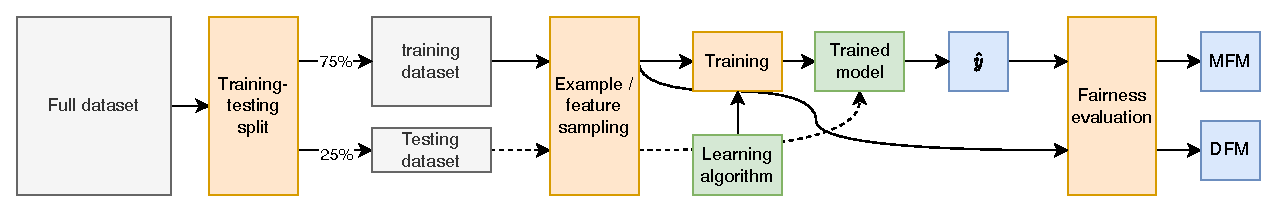
\includegraphics[width=0.95\linewidth]{method.pdf}
  \caption{Methodology for data collection and analysis}
  \label{fig:method}
\end{figure*}

We extend the above experiment further in two ways by adopting the
experimental design from \citeauthor{zhang2021ignorance}. First, we
experiment with different number of training examples and second with
different number of features in the training set. For both
experiments, we shuffle the order of the examples in the training and
testing sets. For the feature sets experiment, we additionally shuffle
the order of the features. For the training sets experiment, we
generate different training samples of varying sizes starting from
10\% until 100\%. For the feature sets experiment, we start with a
minimum of 3 features (in addition to the protected attribute and
target) and introduce one new feature until all the features are
utilised. Both the training and testing sets undergo the same feature
sampling procedure in the feature sample size experiment since the
number of features in the training and testing sets must be the same.
No such sampling is done in the testing set for the training sample
size

\begin{table}
  \centering
  \begin{tabular}{lr}
    \toprule
    \textbf{Parameter} & \textbf{Count}\\
    \midrule
    Fairness metrics & 2\\
    ML models & 4\\
    Datasets & 8\\
    Total cases & $8\times4=32$\\
    Iterations & 50\\
    Total fairness evaluation cycles & $32\times50=1600$\\
    \bottomrule
  \end{tabular}
  \label{tab:parameters}
  \caption{Parameters of the study}
\end{table}

We use Spearman Rank Correlation to quantify the linear relationship
between the DFM and MFM. We use Spearman correlation since it does not
assume normality in the distributions and is less sensitive to
outliers. We repeat all experiments 50 times and use hypothesis
testing to verify the statistically significant of our results. We
report the statistical significance of our results at three $\alpha$
levels of 0.01, 0.05 and 0.1. For simplicity, we represent the
statistical significance using asterisks where more number of
asterisks indicates lower $pvalue$ and thus higher statistical
significance. Note that although the statistical significance is
reported at 3 $\alpha$ levels, we only consider cases where
$\alpha\le0.05$ to be statistically significant in our evaluation.

Table \ref{tab:parameters} summarises the parameters of the study. We
train 4 ML models on 8 datasets producing 32 total cases. The fairness
for each case is evaluated 50 times using two fairness thus producing
a total of 1600 training and fairness evaluation cycles.

\section{Results}\label{sec:results}

This section presents the analysis of the relationship between DFM and
MFM. The section is broken into two subsections.
Section \ref{sec:results-full} presents the relationship between DFM
and MFM as the distribution of the training data changes while
Section \ref{sec:results-training-feature-sets} presents results when
the training sample and feature sample size changes. Where applicable,
each section is further broken down using research questions.

% - Results. in the text we refer to training size of 60%, 50% etc. The
% figures mention frac 0.5, 0.6. Opt for a single way to describe and be
% consistent

\subsection{Full Training Set Experiment}\label{sec:results-full}
\subsubsection{What is the relationship between DFM and MFM?}\label{sec:results-full-rel}

\begin{figure}
  \centering
  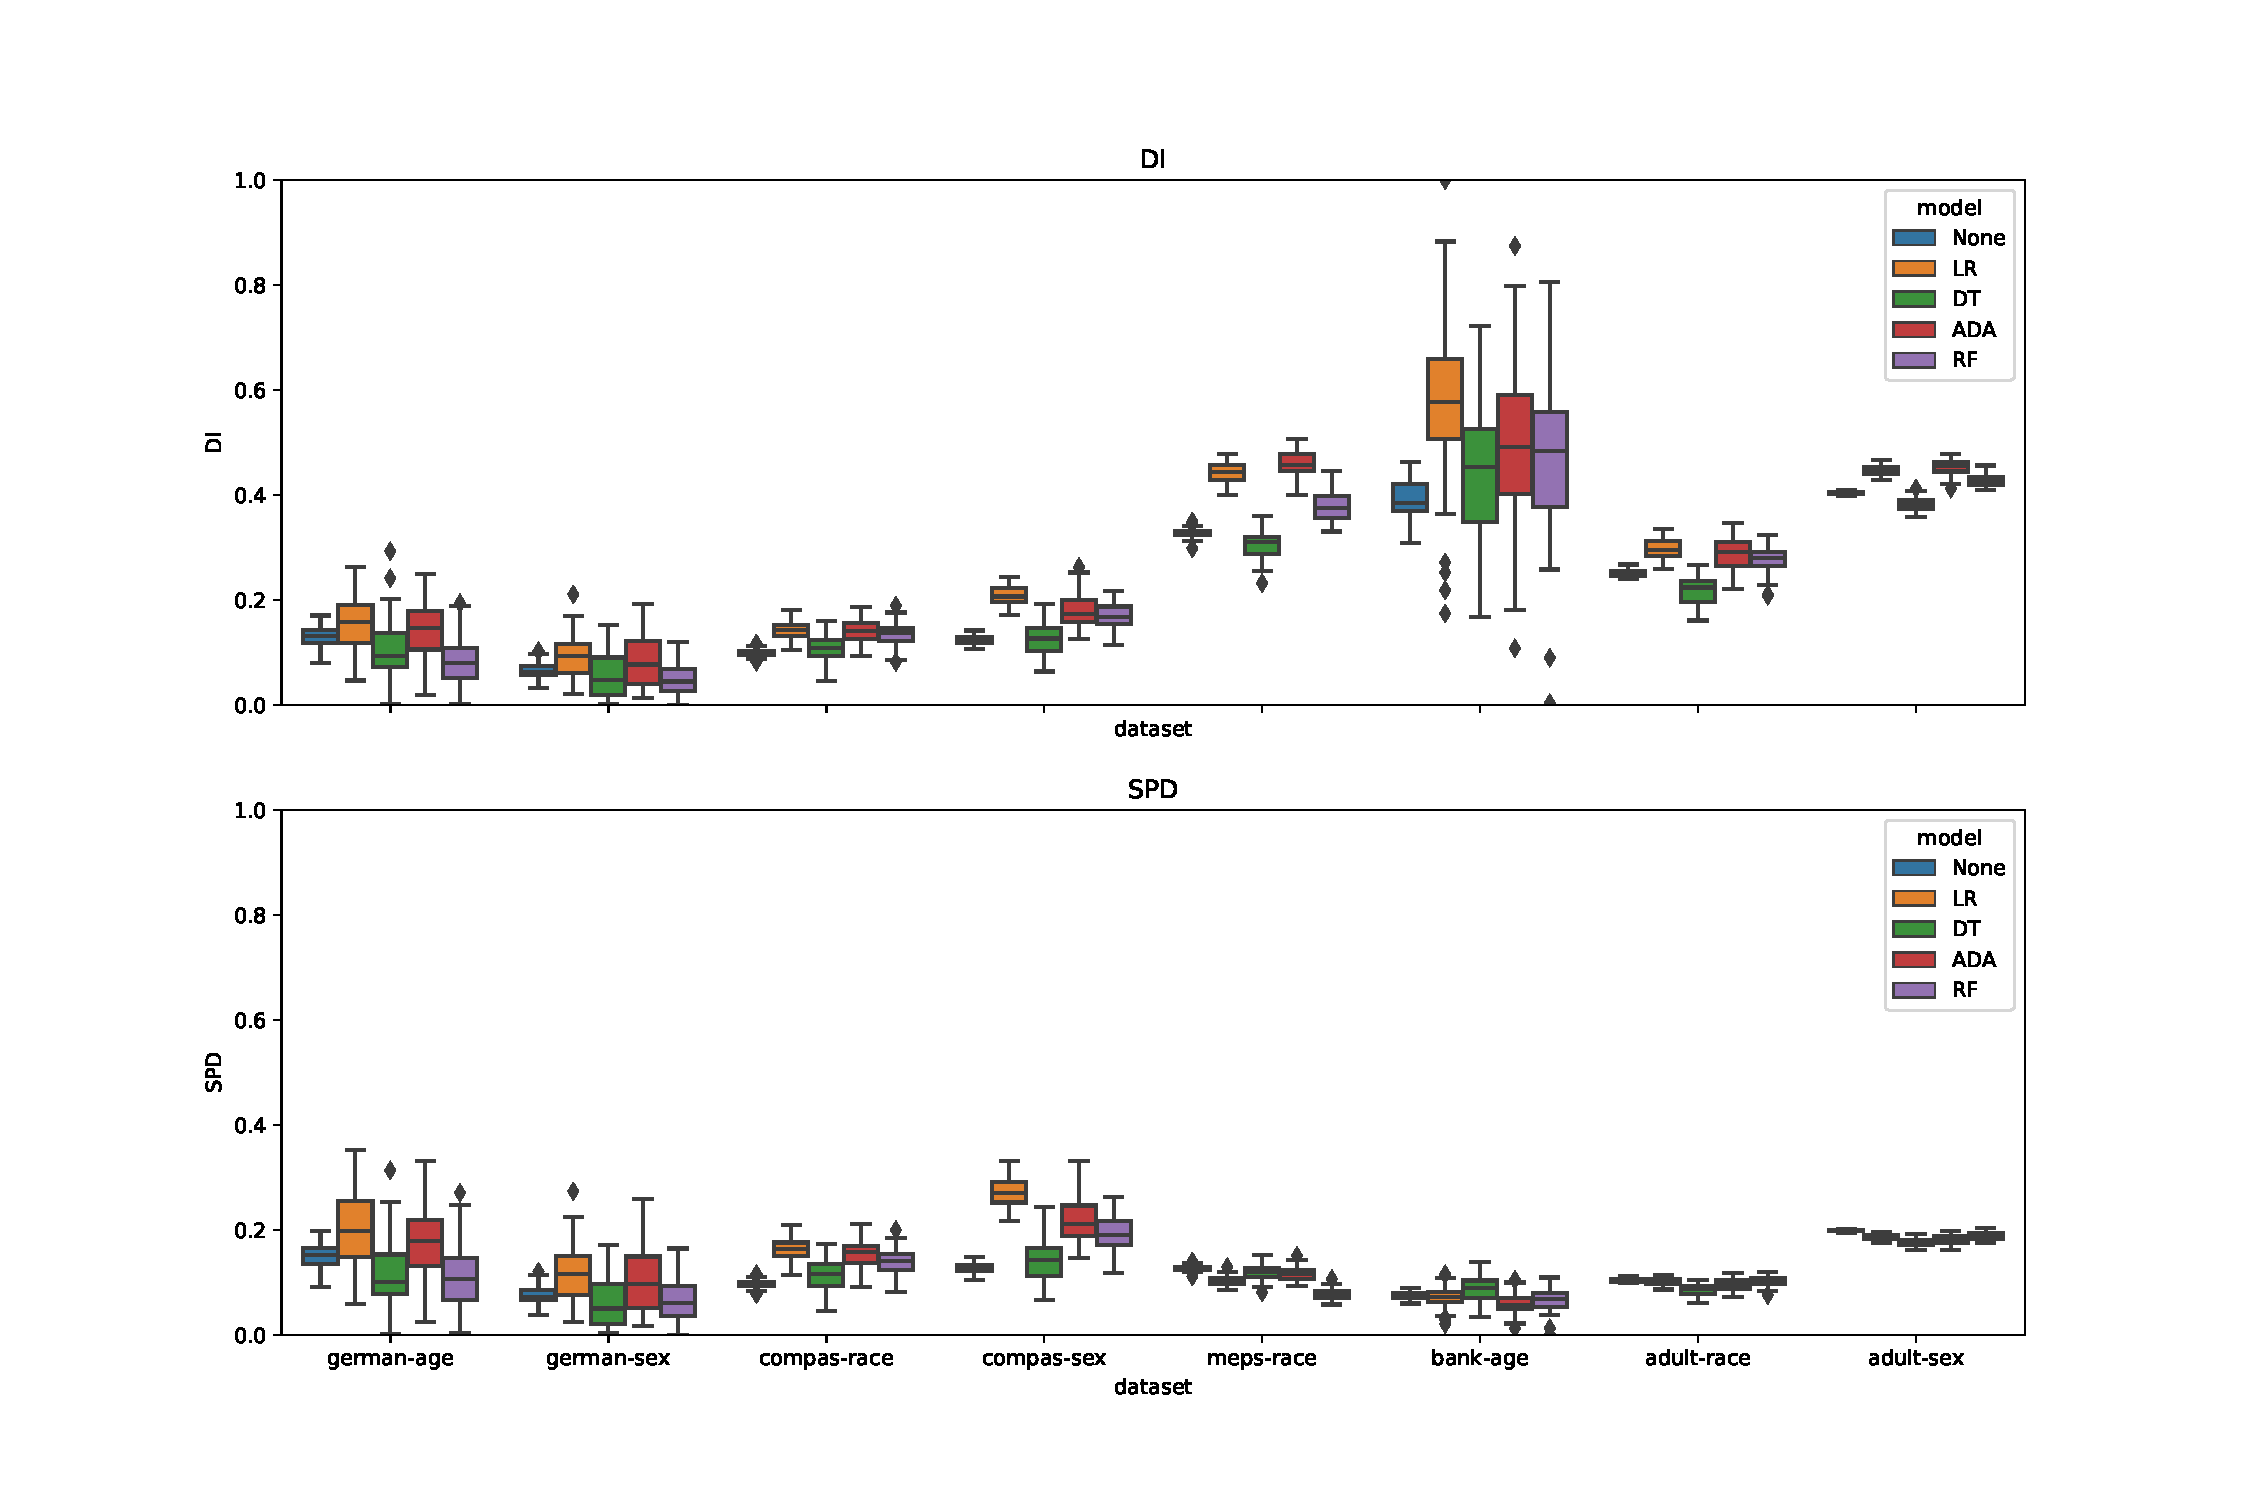
\includegraphics[width=0.95\linewidth]{boxplot--dataset--di-spd--exp-full.pdf}
  \caption{Distribution of DFM and MFM across datasets}
  \label{fig:boxplot--dataset--di-spd--exp-full}
\end{figure}

Figure \ref{fig:boxplot--dataset--di-spd--exp-full} presents a boxplot
with the distribution of the fairness metrics across the datasets. The
x-axis represents the datasets used in this study while the y-axis
presents the value of the fairness metric. The models used in this
study are represented using different colors. Both the fairness
metrics DI (top) and SPD (bottom) are presented in separate plots. We
observe that DFM and MFM convey similar information in all cases. The
variability of the DFM is less than the MFM. This is because
in addition to the randomness from the data shuffling in the training
set, the models are assigned random initial states in every iteration.
Finally in several cases the tree based classifiers (DT and RF) make
fairer decisions compared to the other classifiers, sometimes even
better than the baseline provided by the DFM.

\begin{figure}
  \centering
  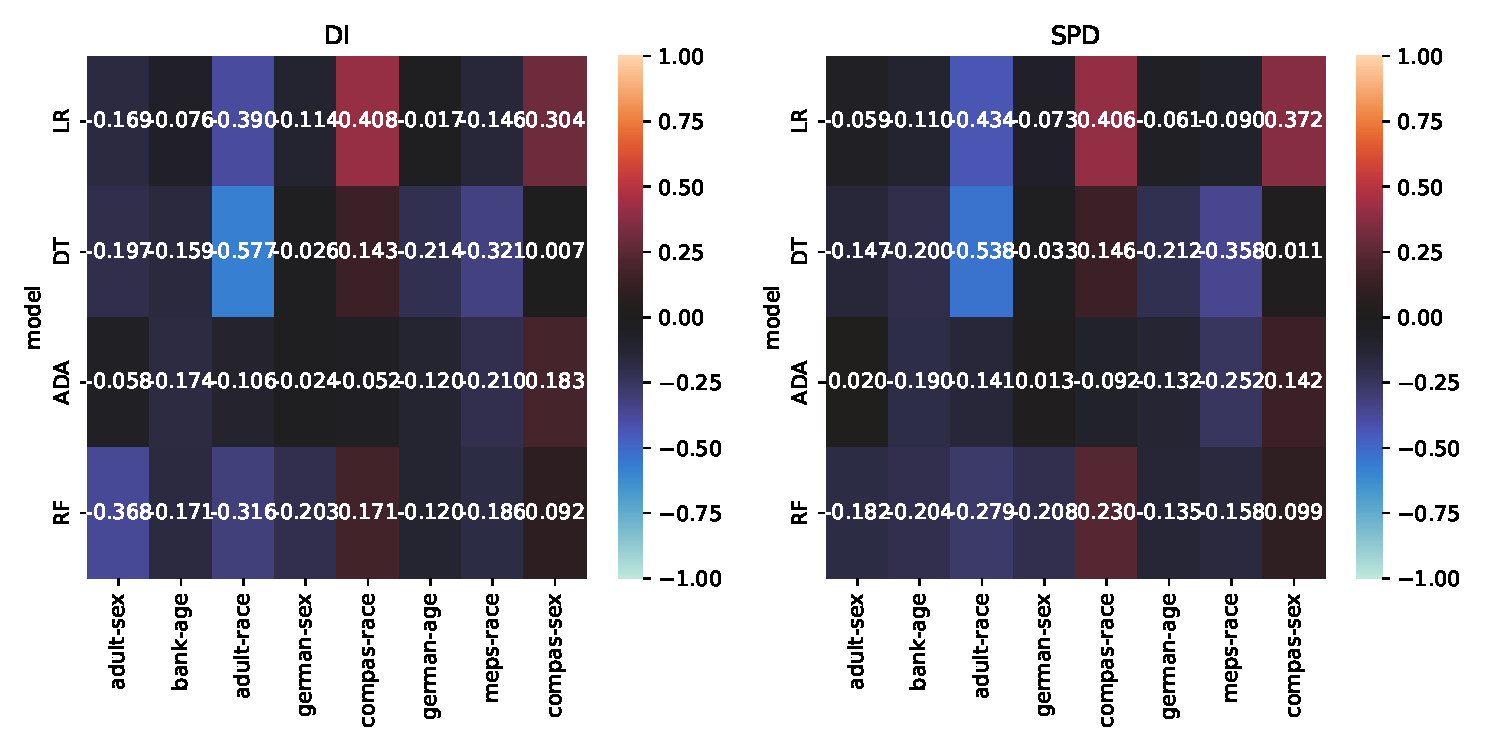
\includegraphics[width=0.95\linewidth]{heatmap--corr--full-data.pdf}
  \caption{Correlation between DFM and MFM. ***: $p\le0.01$; **:
  $p\le0.05$; *: $p\le0.1$}
  \label{fig:heatmap--corr--full-data}
\end{figure}

Figure \ref{fig:heatmap--corr--full-data} presents a heatmap that
shows the correlation between DFM and MFM across all models (along
y-axis) and datasets (along x-axis). Darker colours indicate weaker
correlation whereas brighter colours indicate stronger
correlation. Positive correlation is indicated using hues of red while
negative correlation is indicated using hues of blue. The correlation
between DFM and MFM for both fairness metrics are shown separately. We
primarily observe darker colours in the heatmap indicating that there
is no correlation between the DFM and MFM in most of the cases. The
distribution of the training dataset changes every iteration since we
shuffle the order of the examples prior to creating the training and
testing sets. However this is not enough to produce a significant
quantity of change and thus consequently no correlation amongst the
DFM and MFM.

\subsubsection{How does change in the distribution of the training set
  affect the relationship between DFM and MFM?}\label{sec:results-full-rel-dist}

\begin{figure}
  \centering
  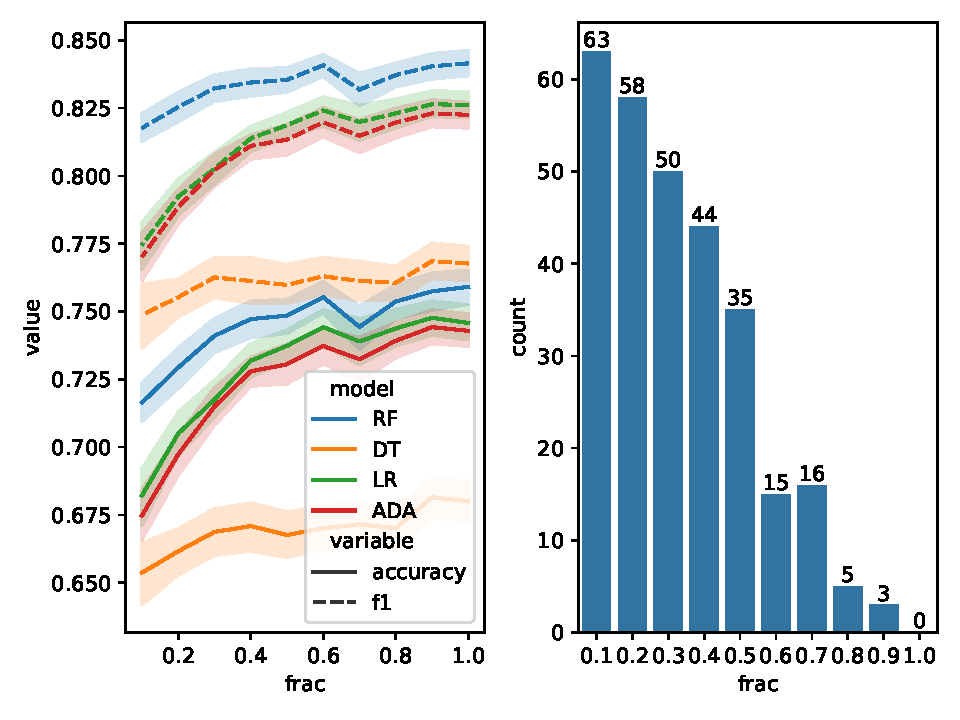
\includegraphics[width=0.95\linewidth]{training-set-frac-threshold.pdf}
  \caption{\emph{\textbf{(left)}} Accuracy and f1 across various
    training sample size in german-age \emph{\textbf{(right)}} Number
    of cases with significant change in accuracy and f1}
  \label{fig:training-set-frac-threshold}
\end{figure}

As seen in Section \ref{sec:results-full-rel}, there is no significant
linear relationship between DFM and MFM due to the lack of significant
change in the distribution of the training dataset across the 50
iterations. To analyse the relationship between the DFM and MFM across
various data distributions, we modify our experimental design by
calculating the DFM and MFM across training samples of varying size.
The data distribution in smaller training samples will change more
frequently in the 50 iterations at the loss of data quality. To
identify a sample size that captures a variety of data distribution
changes while also being a realistic training dataset, we analyse the
\emph{accuracy} and \emph{f1 score} of the models across the training
sample sizes. Next we conduct \emph{student t-test} to identify the
smallest sample size where the performance of the models is similar to
that obtained when trained using the full training set.

Figure \ref{fig:training-set-frac-threshold} (right) presents
a histogram of the number of cases where there was a significant
difference between the two populations. We note that there is
a significant difference in the performance of the models in majority
of the cases when the training size is reduced to 50\% while it
remains consistent when using a training size of 60\% or higher. This
is also corroborated by the lineplot in
Figure \ref{fig:training-set-frac-threshold} (left) which shows the
accuracy and f1 of all models across various training sample sizes in
the \emph{german-age} dataset. We observe that the performance
stabilities starting from 60\% training sample size. Thus for majority
of the cases, a training sample of 60\% allows us to train models with
acceptable performance, while also capturing a wide variety of
fairness issues in the underlying training data within the 50
iterations.

\begin{figure}
  \centering
  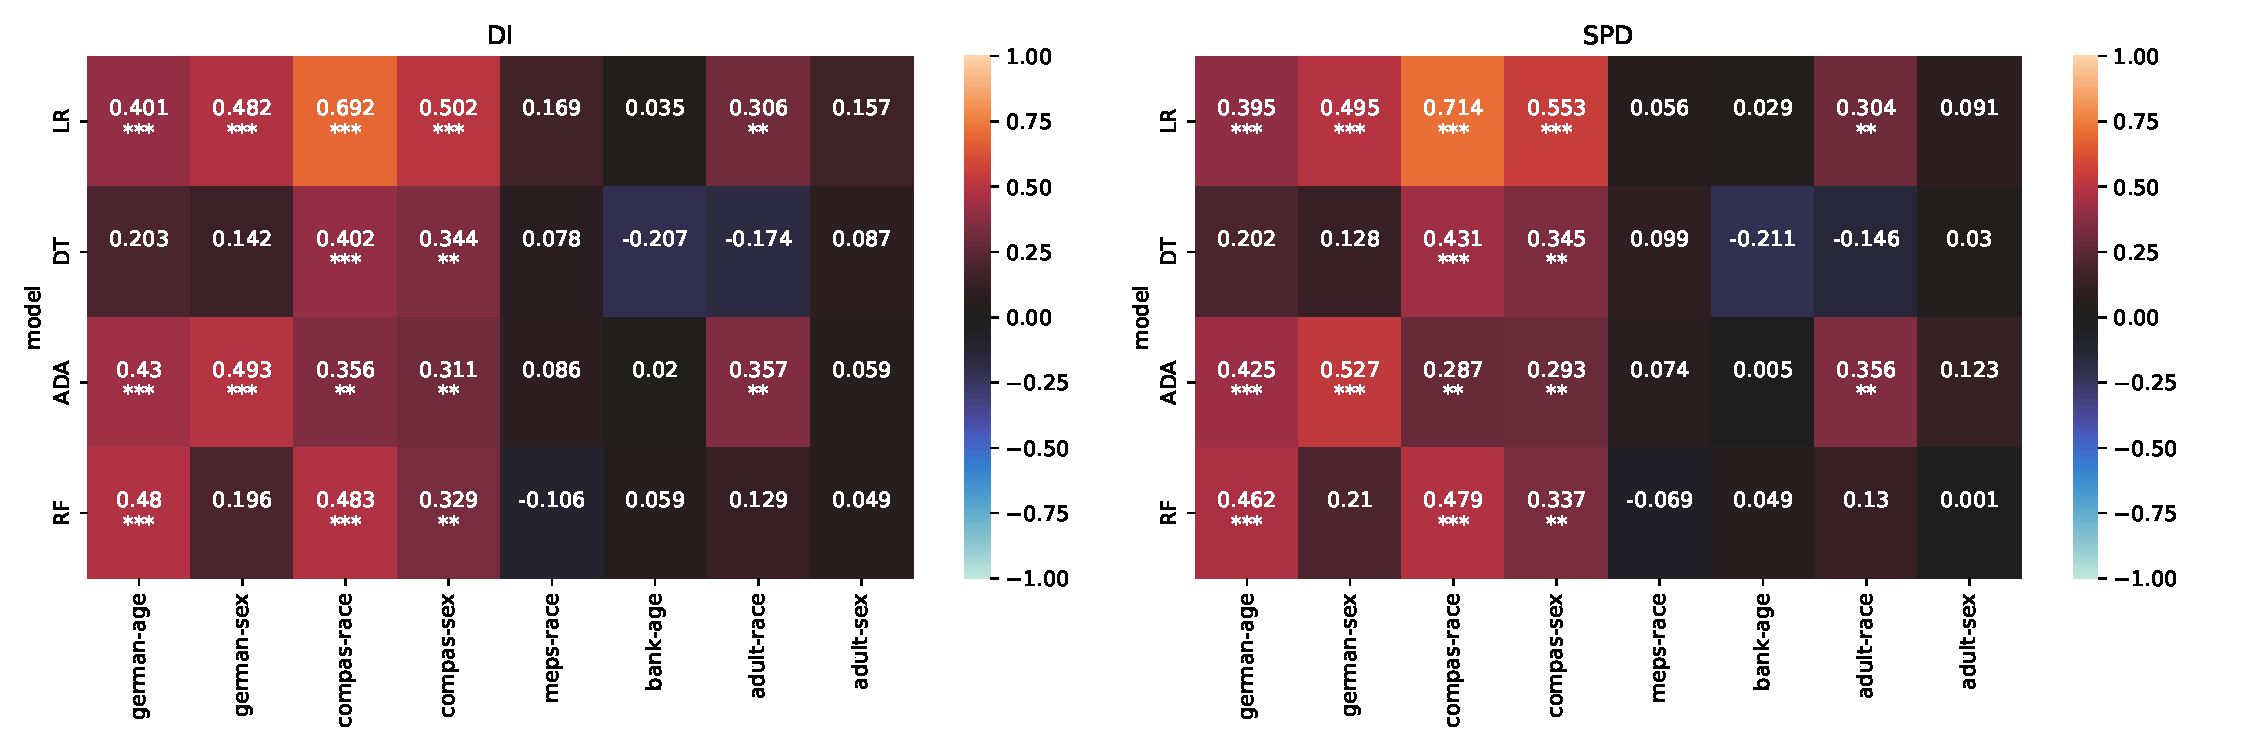
\includegraphics[width=0.95\linewidth]{heatmap--corr--training-sets-frac.pdf}
  \caption{Correlation between DFM and MFM across all models and
  datasets using 60\% training data. ***: $p\le0.01$; **: $p\le0.05$;
  *: $p\le0.1$}
  \label{fig:heatmap--corr--training-sets-frac}
\end{figure}

Figure \ref{fig:heatmap--corr--training-sets-frac} shows the
correlation between the DFM and MFM across all models and datasets
when trained using 60\% of the original training set. In contrast to
Figure \ref{fig:heatmap--corr--full-data}, we primarily observe
a positive correlation between the DFM and MFM. This indicates that
the DFM and the MFM convey the same information as the distribution of
the underlying training dataset changes.

\subsubsection{How does the training sample size affect the correlation between DFM and MFM?}\label{sec:results-corr-frac}

\begin{figure}
  \centering
  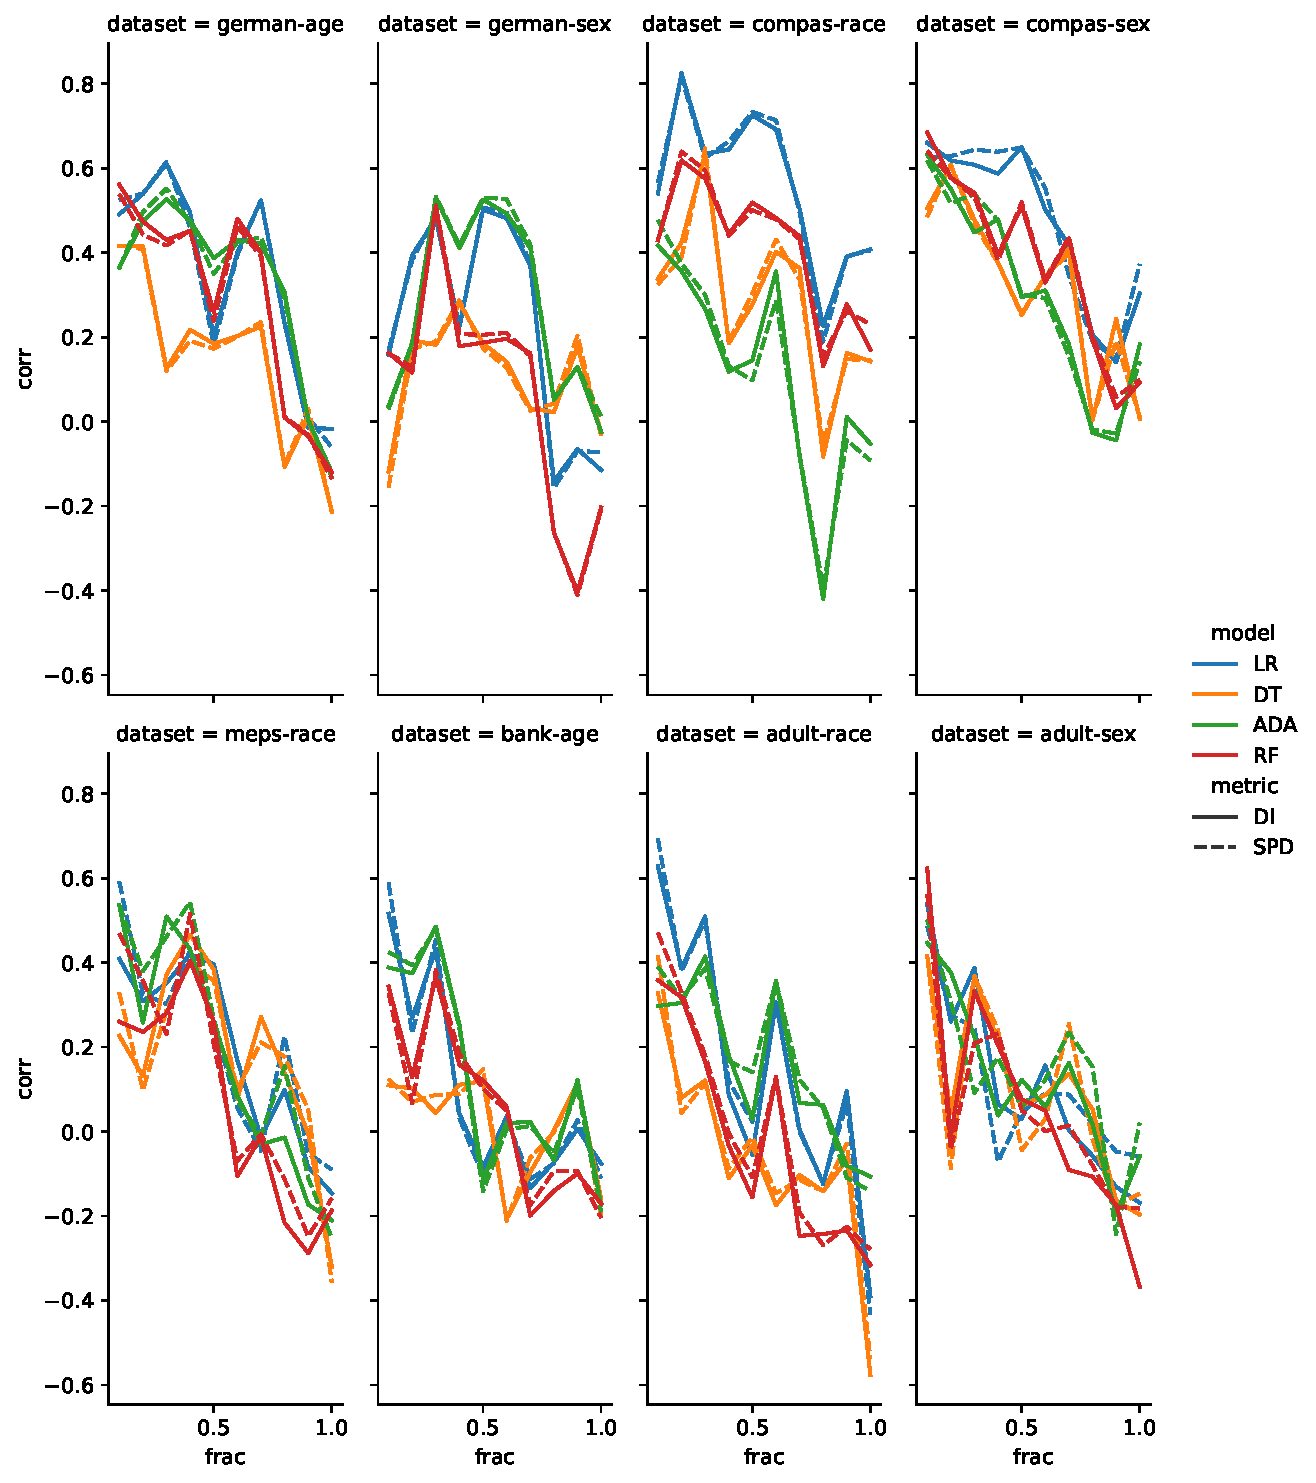
\includegraphics[width=0.95\linewidth]{lineplot--frac--corr.pdf}
  \caption{Distribution of correlation between DFM and MFM across
    various training sample sizes}
  \label{fig:lineplot--frac--corr}
\end{figure}

In Figure \ref{fig:heatmap--corr--full-data} we observe that the
smaller datasets have no correlation between DFM and MFM while the
larger datasets show a negative correlation. When we reduce the
training sample size to 60\%, the correlation in the smaller datasets
become more positive while the larger datasets do not show any
correlation as seen in
Figure \ref{fig:heatmap--corr--training-sets-frac}. Based on these
observations, we hypothesise that the quantity of training data
influences the fairness of the model. Our hypothesis is corroborated
by Figure \ref{fig:lineplot--frac--corr} which shows the distribution
of the correlation between DFM and MFM across the training sample
sizes in all datasets and models. The x-axis presents the training
sample size and the y-axis presents the correlation between DFM and
MFM. The colours represent the models while the style of the line
represent the two fairness metrics. Each dataset is represented as
a separate subplot. The overwhelming majority show that the
correlation between the DFM and MFM decreases as we increase the
training size.

\subsection{Training and Feature Sets
  Experiments}\label{sec:results-training-feature-sets}
In addition to the analysis presented above, we extend the analysis
conducted by \citeauthor{zhang2021ignorance} by evaluating the effect
of training and feature sample size on the relationship between DFM
and MFM.

\subsubsection{What is the relationship between DFM and MFM across
  various training samples?}\label{sec:results-training-sets}

\begin{figure}
  \centering
  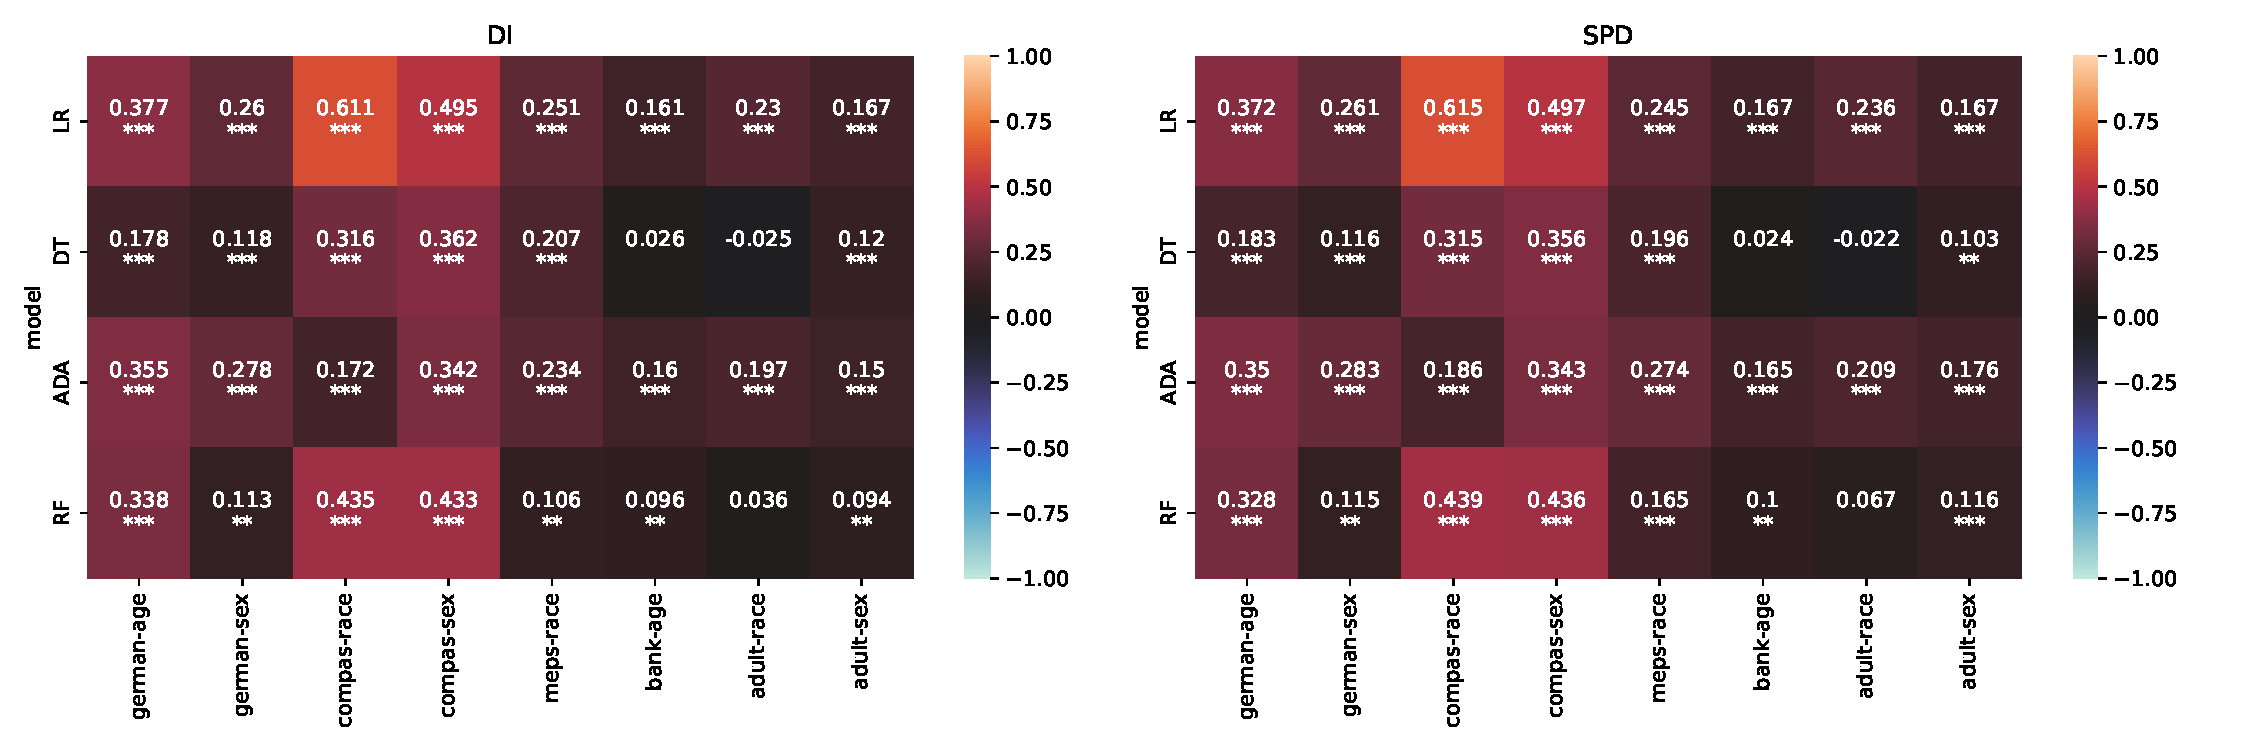
\includegraphics[width=0.95\linewidth]{heatmap--corr--frac.pdf}
  \caption{Correlation between DFM and MFM acoss various training
  sample sizes. ***: $p\le0.01$; **: $p\le0.05$; *: $p\le0.1$}
  \label{fig:heatmap--corr--frac}
\end{figure}

In this section we analyse the relationship between DFM and MFM across
varying training sample sizes. In contrast to
Section \ref{sec:results-corr-frac} where we calculated the
correlation between DFM and MFM within the specific training sample
sizes, here we calculate the correlation across all training sample
sizes. Figure \ref{fig:heatmap--corr--frac} shows the correlation
between DFM and MFM across various training sample sizes. We primarily
observe colours indicating that the DFM and the MFM convey similar
information.

\subsubsection{What is the relationship between DFM and MFM across various feature samples?}\label{sec:results-feature-sets}

\begin{figure}
  \centering
  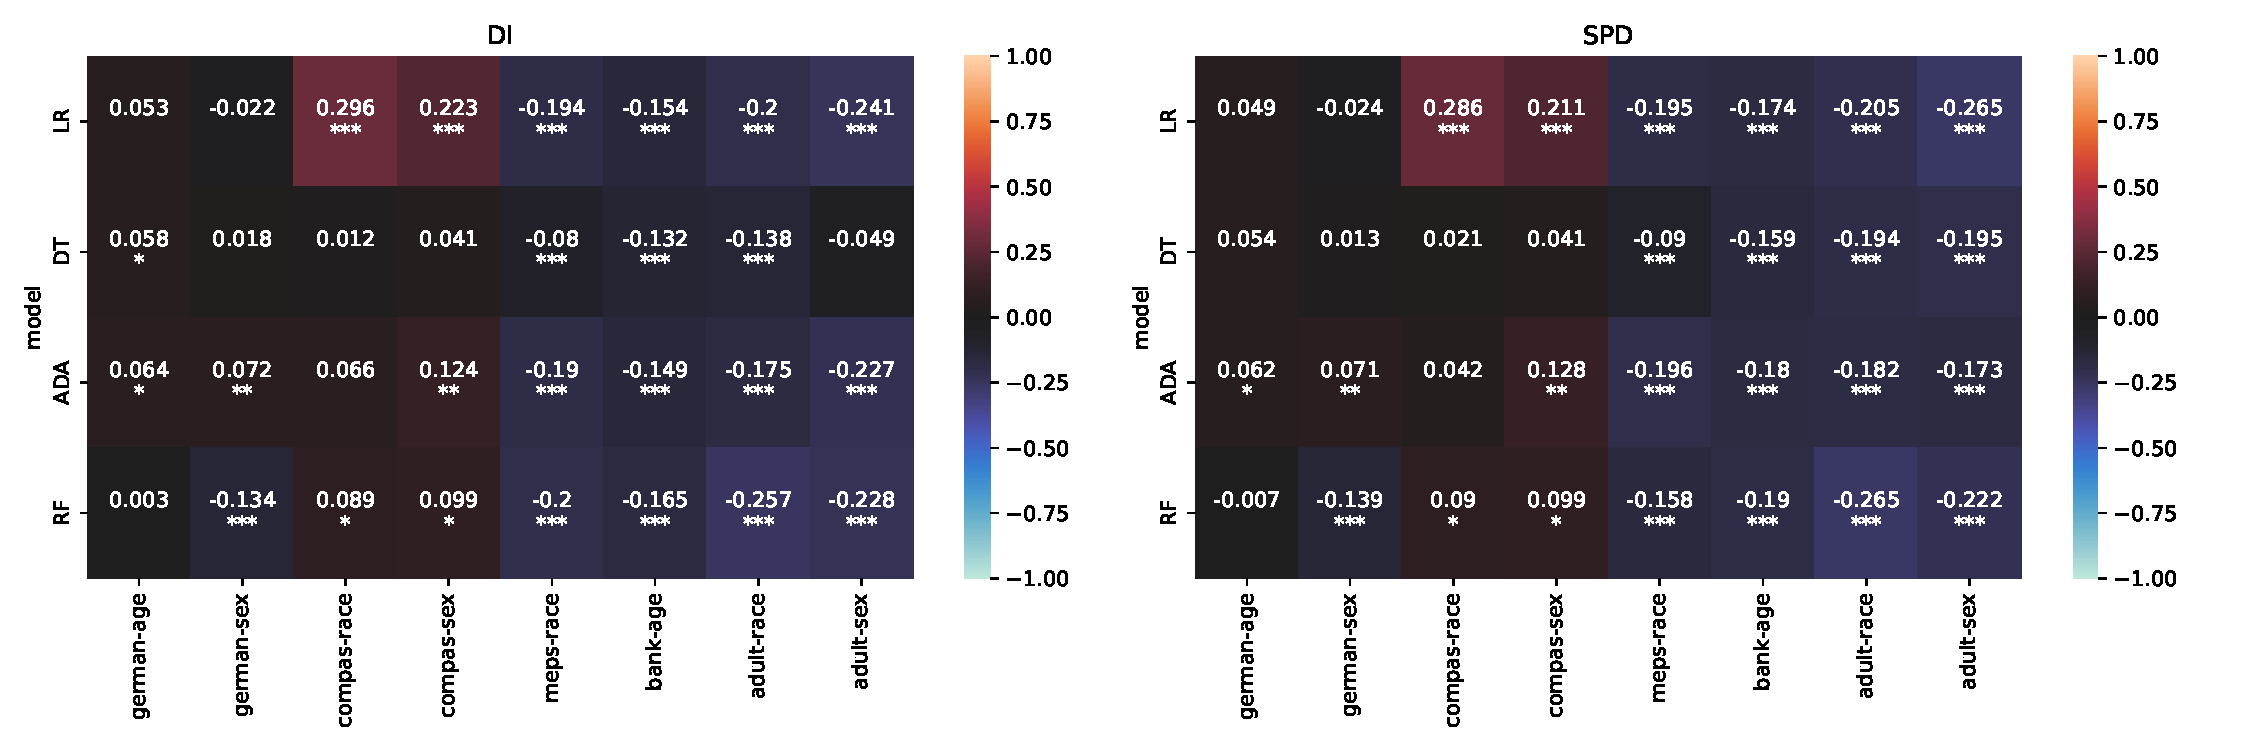
\includegraphics[width=0.95\linewidth]{heatmap--corr--num-features.pdf}
  \caption{Correlation between DFM and MFM across various feature
  sample sizes. ***: $p\le0.01$; **: $p\le0.05$; *: $p\le0.1$}
  \label{fig:heatmap--corr--num-features}
\end{figure}

In this section we analyse the relationship between the DFM and MFM
across varying feature sample sizes. In contract to
Section \ref{sec:results-training-sets}, we change the number of
features in the training set and randomise the feature order in each
iteration. Figure \ref{fig:heatmap--corr--num-features} presents the
correlation between the DFM and MFM across all feature sample sizes.
We primarily notice darker colours indicating that there is no
significant correlation between the DFM and MFM as the number of
features in the training dataset changes.

From Equation \ref{eq:di-data} and \ref{eq:spd-data}, we note that
feature sample size does not affect the DFM thus explaining the lack
of significant correlation between the DFM and MFM. The larger
datasets show a more negative correlation. This however is due to the
change in training set distribution caused by the training-testing
split within the 50 iterations as explained
in Section \ref{sec:results-full}. This can also be verified in
Figure \ref{fig:lineplot--num-features--corr} which shows the
relationship between the correlation and the feature sample sizes
across all datasets and models. There is no discernible relationship
between the correlation and the feature sample size in the top row
containing datasets with a small training sample size but large
feature sample size. In contrast, a slight relationship can be observed
in the bottom row which contains datasets with a larger training
sample size but smaller feature sample size.

\begin{figure}
  \centering
  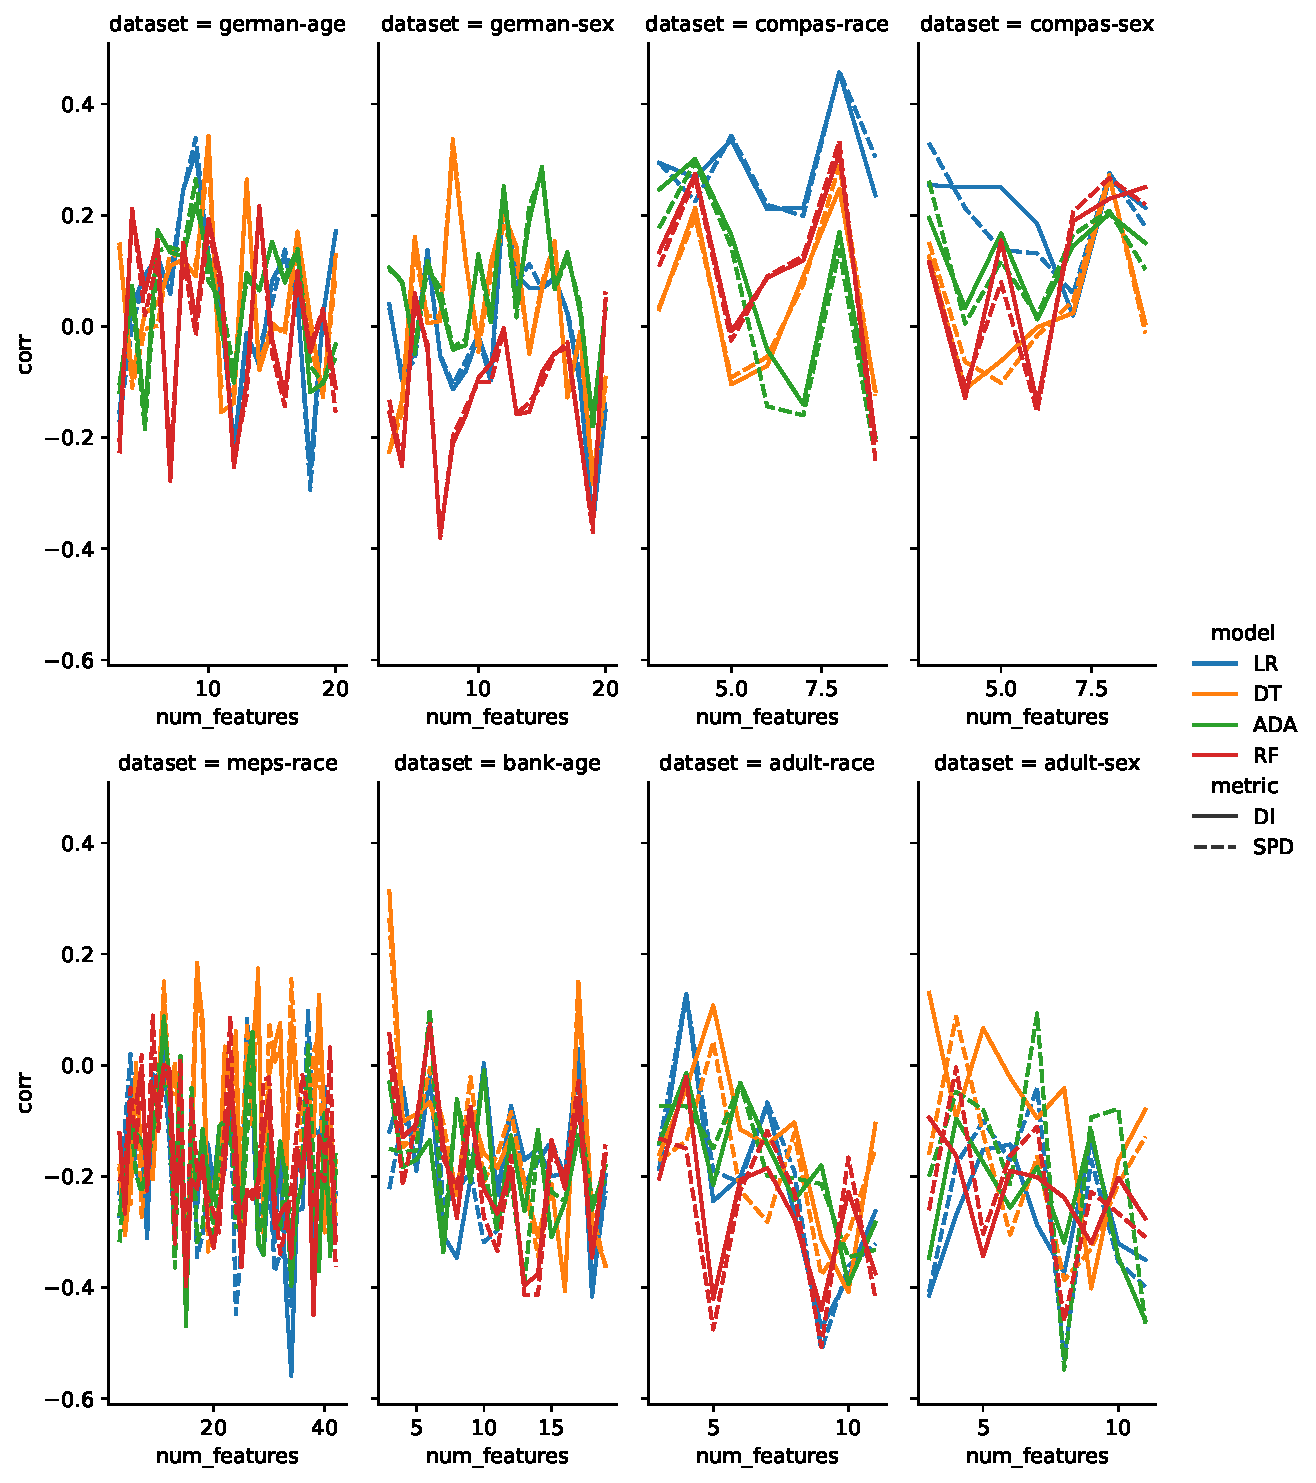
\includegraphics[width=0.95\linewidth]{lineplot--num-features--corr.pdf}
  \caption{Distribution of correlation between DFM and MFM across
    various features sample sizes}
  \label{fig:lineplot--num-features--corr}
\end{figure}

\section{Discussion}\label{sec:discuss}

% % - " Zhang and Harman showed that the feature sample size has
% profound effect on the fairness of the ML model, where larger
% feature sample sizes typically improve the models ability to make
% fairer predictions [Zhang and Harman, 2021]."

% - Saying this seems
% like we are discussing the implications of their results. I would
% just say whether our findings agree or disagree with their
% work. 

% - I like the main idea of the paragraph.  can we say something
% about the importance of feature selection and that feature selection
% techniques should not be fairness agnostic? I.e., it's not only
% about extracting the features with more predictive power but also
% the ones that ensure fairness in the model

% Since we recommend that testing fairness before and after training,
% we could also say that we need metrics that can be applied before
% and after training. I.e., if we have different metrics before and
% after, we are complicating things for practitioners ;)

% Another remark that might be interesting is the need of more
% empirical studies to understand how these metrics can actually be
% applied in real projects. Something around the lines of going from
% theory to practice

\subsection{Locating root cause of bias}\label{sec:discuss-root-cause-bias}

%% DFM are so "cheap"; computationally there is practically no
%% overhead & it avoids a full training cycle!
Our results indicate the importance of testing for fairness in ML
systems both before and after training. Testing for fairness only
after training the model makes it very difficult to identify where
exactly the bias was introduced. Thus, a holistic view of the entire
system is necessary to aid practitioners locate the root cause of
bias. Testing for fairness both at the data (using DFM) and model
(using MFM) levels gives us some lead in identifying the root cause of
bias. If the DFM indicates presence of bias, it can be an early
indication of flaws in the data collection or alternatively in the
initial design of the system itself. In the event that the DFM does
not indicate bias but the MFM does indicate bias, practitioners can
narrow down the cause of bias to the learning algorithm itself and opt
for in-processing or post-processing bias mitigation techniques.

%% DFM are computationally ``cheap'' and can help identify root cause of
%% bias early which can lead to significant reduction in the development
%% time.

%% %% mention that detecting root cause early can lead to significant dev
%% time reduction -> cost effective & better for developer
%% productivity.

\subsection{Fairness, efficiency and performance trade-off}\label{sec:discuss-fair-eff-perf-trade}

Our results indicate that the quantity of training data profoundly
influences the relationship between DFM and MFM. We primarily see a
positive correlation between the DFM and MFM in smaller training
samples which indicates that the DFM and MFM convey the same
information. With sufficient training data, the correlation starts to
drop and eventually becomes negative. This indicates that the models
learn to make fairer predictions and are able to circumvent the bias
in the training data to a certain extent.
%% feffer2022empirical may be a relevant cite here; they comment on
%% volatility of train-test splits & how ensembling techniques can
%% mitigate this volatility

% TODO refactor this sentence; too complex
Same information from the DFM and MFM---specifically, when both DFM
and MFM are high indicating presence of bias and potential fairness
issue---may indicate lack of sufficient training data. Under such
circumstances, practitioners can either choose to collect more data if
possible else use bias mitigation techniques to address the fairness
issue. A negative correlation between DFM and MFM may arise from two
possibilities: either the MFM is higher than the DFM (discussed in
Section \ref{sec:discuss-root-cause-bias}) or the MFM is lower than
the DFM which is what we analyse here. A lower MFM value compared to
the DFM merely indicates that the biases in the data is no longer
reflected by the model. However, there may yet be bias in the model
from other sources. \citeauthor{zhang2021ignorance} showed that in
addition to the quantity of training data, the quality itself affects
the fairness of ML systems. Introducing more data does not always fix
the bias in the model if the data remains biased.

Lower MFM compared to DFM also presents a trade-off between efficiency
and performance. A slight reduction in the training sample size, in
combination with appropriate bias mitigation techniques, can allow
practitioners to build fair ML systems with quicker training cycles at
the cost of negligible predictive performance \cite{verdecchia2022data}.
Engineering efficient, high quality training data can reduce training
cycles, time and ultimately project costs. Compounded over the entire
duration that an ML system stays in production along with the human
effort required to keep such a system operational, the benefits can be
more than substantial.

No correlation between DFM and MFM presents a trade-off between
fairness, efficiency and performance. Practitioners may opt for a more
efficient system by reducing the training sample size. However this
may reduce the predictive performance of the model and require more
engineering effort to mitigate the fairness issues in the system.
Alternatively, they may opt for more accurate predictions by using a
larger training sample size. A larger training size may mitigate some
of the bias in the training set at the cost of more compute.

\subsection{Data Drift}\label{sec:discuss-data-drift}

Results from experiments conducted in Section \ref{sec:results-full}
indicate that the DFM can be an early indication of fairness issues
that may manifest in the ML models when the distribution of the
training data changes. ML systems running in a production environment
are often monitored to detect degradation in model performance. A
standard practise is to combine the data encountered by the model in
the production environment with its predictions to create the training
set for the next
iteration \cite{biessmann2021automated,breck2019data,schelter2018automating}.
Since data reflects the real world, change in its underlying
distribution over time is eminent. Our results indicate that DFM can
also be used as a early warning system to identify fairness related
data drifts in automated ML pipelines.

\subsection{Test Reduction}\label{sec:discuss-test-red}

Experimentation with the size of the training set (sampling) and
features of the training set (feature engineering) is a popular
practise when engineering ML pipelines. Results from
Section \ref{sec:results-training-feature-sets} indicate that the DFM
and MFM are positively correlated and thus convey the same information
when the training sample size changes. This implies that when
experimenting with the training sample size, ML practitioners can
reduce their fairness testing efforts to just the data and avoid a
full training cycle. Compounded over the duration that an ML system is
operational, along with the multiple iterations it takes to test an ML
system, avoiding a full training cycle while evaluating the fairness
of the ML system can be very energy efficient and sustainable in the
long run.

%% if we can find a paper that shows that the churn rate for training
%% size is more than feature size; then we can back our findings a bit
%% more

Our results however also indicate that the same test reduction cannot
be made when experimenting with the feature sample size of the
training set. \citeauthor{zhang2021ignorance} showed that the feature
sample size has profound effect on the fairness of the ML model, where
larger feature sample sizes typically improve the models ability to
make fairer predictions \cite{zhang2021ignorance}. To the best of our
knowledge, there are no fairness metrics that consider the influence
of other features on the fairness at the data level. Thus when
experimenting with the feature set, it is recommended that ML
practitioners evaluate the fairness at both before and after training.

\subsection{Explaining fairness in decision trees}\label{sec:discuss-explain-fair-dt}

From our analysis, we consistently observe that Decision Trees (DTs)
are able make fairer predictions with minimal effort. For instance, in
Figure \ref{fig:boxplot--dataset--di-spd--exp-full} we observe that
DTs report lower values for both fairness metrics across all datasets.
In Figure \ref{fig:lineplot--frac--corr} we observe that DTs
consistently report lower correlation between DFM and MFM compared to
other models. This indicates that DTs are able to mitigate the bias
present in the training data with a smaller training sample size and
continue to do so as the training same size varies. The above
observations pose an interesting line of query into examining why DTs
are able to produce fairer predictions using explainable AI
techniques.
%% we need to improve by citing relevant explainable AI papers here.

\section{Threats to Validity}\label{sec:threats}

We use the spearman correlation implementation provided by
scipy \ref{virtanen2020scipy} python library. The $pvalue$ provided by
the current implementation however is not reliable for population size
less than 500 experiments\footnote{See notes in the
\href{https://docs.scipy.org/doc/scipy/reference/generated/scipy.stats.spearmanr.html}{library
  documentation}}. This is a threat to the experiments conducted in
Section \ref{sec:results-full} since we only have 50 samples. For
these experiments, we additionally conduct linear regression analysis
using ordinary-least squares and check the coefficient of
determination ($R^2$) and the mean squared error (MSE) in the
residuals to evaluate the goodness of fit. We set the MFM as the
outcome (or dependent) variable $y$ and the DFM as the design (or
independent) variable $x$. The linear regression results align with
our findings from the correlation analysis. For the experiment in
Section \ref{sec:results-full-rel}, the $R^2$ in majority of the cases
lie close to 0 indicating that the linear regression model is unable
to explain the variability in the MFM using the DFM. For the
experiment in Section \ref{sec:results-full-rel-dist}, the $R^2$
improves relative to the prior experiment thus reflecting the change
we also observe in the correlation analysis.

% domain expertise: we restricted our analysis to 2 group fairness
% metrics; there are several others but they focus on evaluating the
% fairness of the model (need y_hat); domain expertise is also
% required to evaluate effectiveness of the type of fairness itself!
% we used group fairness is it is easy to comprehend (by humans) and
% most widely used in practise & literature

%% lack of correlation may arise from lack of significant bias in the
%% dataset; thus the DFM and MFM are just random and will never be
%% related; see german-sex for example

%% revisit this paragraph; last sentence needs to be smoother around
%% the edges...
For the experiment conducted in
Section \ref{sec:results-full-rel-dist} the selection of the training
sample size of 60\% is a gross approximation and may not be a good fit
for all datasets used in this study. An alternative albeit
computationally more expensive solution would be to identify this
threshold dynamically individually for each dataset. Although this may
lead to different results in the correlation analysis, we believe that
the final outcome and insights will remain the same.


%% TODO we did not look at the underlying distribution of the training
%% dataset (which is biased to begin with); it will be interesting to
%% evaluate if we can minimize fairness testing when we utilise bias
%% mitigation techniques

\section{Conclusion}\label{sec:conclude}
%% TODO

\bibliographystyle{named}
\bibliography{report}

\end{document}

